\documentclass{standalone}
\usepackage{tikz}
\usepackage{ctex,siunitx}
\setCJKmainfont{Noto Serif CJK SC}
\usepackage{tkz-euclide}
\usepackage{amsmath}
\usetikzlibrary{patterns, calc}
\usetikzlibrary {decorations.pathmorphing, decorations.pathreplacing, decorations.shapes,}

\begin{document}
\small
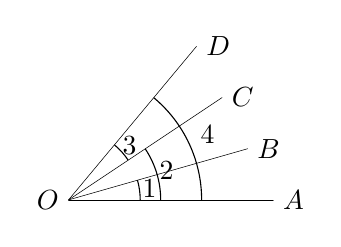
\begin{tikzpicture}[>=stealth,scale=1.3]
  \tkzSetUpPoint[fill=black]
  % \useasboundingbox(-1,-0.75)rectangle(3.7,1.4);
  \tkzDefPoints{0/0/O, 2/0/A, 1.75/.5/B, 1.5/1/C, 1.25/1.5/D}
  \tkzDrawSegments(O,A O,B O,C O,D)
  \tkzLabelPoints[right](A,D,B,C)
  \tkzLabelPoints[left](O)
  \tkzMarkAngles[mark=none, size=.7](A,O,B C,O,D)
  \tkzMarkAngles[mark=none, size=.9](A,O,C)
  \tkzMarkAngles[mark=none, size=1.3](A,O,D)
  \tkzLabelAngle[pos=1.5](A,O,D){4}
  \tkzLabelAngle[pos=1](A,O,C){2}
  \tkzLabelAngle[pos=.8](A,O,B){1}
  \tkzLabelAngle[pos=.8](C,O,D){3}
\end{tikzpicture}
\end{document}